% Do NOT change this "Section" title
% and do NOT add more "Section" level titles.
\section{Implementation}\label{sec:implementation}
Text

\subsection{Gripper}
The gripper have been designed in such a way that it is almost completely retracted in the tool compartment, providing a streamlined and hydrodynamic appearance. Naiad has two grippers installed on the underside of the hull. 

\begin{figure}[h]
    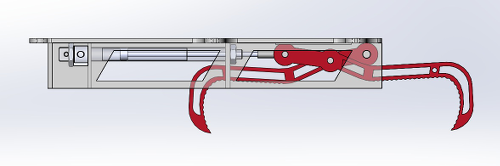
\includegraphics[width=0.5\textwidth]{./figure/gripper_open.png}
    \caption{Gripper at open position}
    \label{fig:one_column_figure}
\end{figure}

In order to grip more effectively, they close with a very wide scooping motion, downwards and to the front. Moreover, the jaws are designed to interlock so they won't open accidentally. Each gripper is actuated by a single-acting naturally retracted cylinder, that in case of a power failure will open automatically (spring return), providing a "dead man's grip" mechanism.

\subsection{Marker}
The marker consists of a sphere attached to a tail ending in a conical shape pointing upwards. When inserted into the bay, this conical shape pushes and locks on a spring loaded latch. The latch is actuated by a single-acting naturally retracted cylinder. There are two marker bays on the vessel.

\begin{figure}[h]
    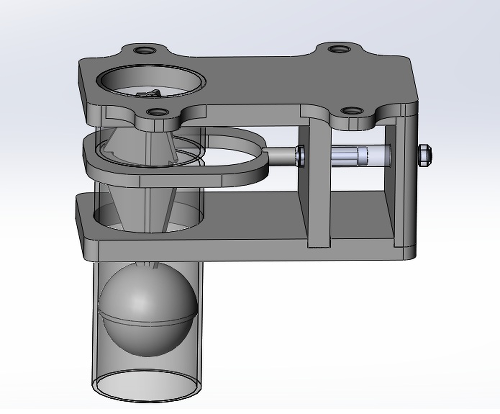
\includegraphics[width=0.5\textwidth]{./figure/marker_loaded.png}
    \caption{A loaded marker}
    \label{fig:one_column_figure}
\end{figure}

\subsection{Torpedo launcher}
There are two torpedo  bays on the front. The torpedoes have been designed to fit precisely in the bays and kept in place by a small spring loaded ball.

\begin{figure}[h]
    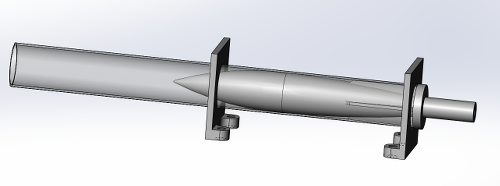
\includegraphics[width=0.5\textwidth]{./figure/torpedo_loaded.png}
    \caption{Torpedo in bay}
    \label{fig:one_column_figure}
\end{figure}

An adjustable burst of air provides propulsion to the desired distance.

\subsection{Gas tank and Valves}
The system is supplied with compressed CO2 by a common 16gr CO2 cartridge. This cartridges are very small and hold an adequate volume of gas. Also they allow a rapid "recharge", simply by replacing the cartridge. Last but not least, they output a constant level of pressure until they are almost completely empty, whereas in compressed air systems, the pressure drops with every actuation.

Leaving from the tank, the gas is passing through a regulator and supplied to a manifold, where it is distributed to the valves. The markers and the grippers will be actuated by four 3-way valves (one for each cylinder). Each torpedo bay will be actuated by a 2-way valve. Safety valves on the tank and the manifold will protect the system and personnel from overpressure.
